\chapter{Design}

\section{Overall System Design}

\subsection{Short description of the main parts of the system}
\textbf{Main Menu}\\
This will consist of a search bar button, an exit button, an add company button and a delete company button.\\
\textbf{Results Page}\\
This will consist of all of the relevant results to the item searched, the search bar in the top right of the window, an Edit information button, an Add information button and a Delete information button.\\
\textbf{Company Information Page}\\
This page will consist of all of the information about the specific company selected. It will show each of the suppliers phone number, owners name, email address, part provided, part price, address and website.\\
\textbf{Comments Section}\\
This page will consist of all the comments other employees have left. It will also have an "add comment" button that allows employees to add new comments.\\

\subsection{System flowcharts showing an overview of the complete system}
\begin{center}
\includegraphics[scale=0.9]{Design_Flowchart.png}
\end{center}
\section{User Interface Designs}

\begin{center}
\includegraphics{UI1.png}
\includegraphics{UI2.png}
\includegraphics{UI3.png}
\end{center}

\section{Hardware Specification}

A computer - desktop or laptop - no specific requirements, must be able to run simple programs\\
A monitor - that shows the program working\\
A keyboard - to be able to use the program\\
A mouse - to be able to use the program\\

\section{Program Structure}
 The main menu will be able to exit the program via a push button. Alternatively it will be able to move to the results page if an item is searched for and is valid. On the results page, the user will be able to add a new supplier into the database via a push button which will take them to the page where they enter the information of the new supplier. Once entered, it will take the user back to the results page. The results page will also allow the user to edit a supplier's information where it will take them to a separate window where they can edit the information already present, or delete the whole data. Once the user is happy with their changes, the program will go back to the results page. The results page will also be able to go back to the main menu if required. Once a supplier has been selected on the results page it will take the user to a new window where the relevent information will be shown. Here they can go back to the results page or click comments to be able to view the comments. On the comments page the user will be able to add a comment or edit/delete comments already made. They will also be able to go back to the information page.

\subsection{Top-down design structure charts}

\begin{center}
\includegraphics[scale=0.6]{topdownthing1.jpg}
\end{center}


\subsection{Algorithms in pseudo-code for each data transformation process}
$FUNCTION SearchDatabase\\
valid = False\\
while valid == False:\\
GET itemtosearch\\
IF itemtosearch is a string:\\
FROM Database\\
SELECT itemtosearch\\
ResultsWindow()\\
valid = True\\
ELSE:\\
print("Item searched is no valid")\\
valid = False\\
$
\newline
$FUNCTION AddSupplier\\
valid = False\\
while valid == False:\\
Get supplierinformation\\
Get partsinformation\\
IF supplierinformation is a string and parts_information is a string:\\
ADD supplierinformation \\
ADD partsinformation\\
valid = True\\
ELSE:\\
print("The data entered is not valid")\\
valid = False\\
$
\newline
$FUNCTION AddComment\\
valid = False\\
while valid == False:\\
Get usercomment\\
Get userrating\\
IF usercomment is a string and user_rating is an integer:\\
ADD usercomment\\
ADD userrating\\
valid = True\\
ELSE:\\
print("Invalid comment")\\
valid = False
$
\subsection{Object Diagrams}

\subsection{Class Definitions}
\begin{itemize}
	\item Employee
	\item Part Needed
	\item Company information
\end{itemize}

\subsection{Class definitions}
\begin{center}
\begin{tabular}{ |c| }
\hline
\textbf{Employee}\\
\hline
FirstName\\
LastName\\
ID\\
\hline
GetUserFirstName\\
GetUserLastName\\
GetUserID\\
\hline
\end{tabular}
\end{center}
\begin{center}
\begin{tabular}{ |c| }
\hline
\textbf{PartNeeded}\\
\hline
PartName\\
PartSize\\
PartPrice\\
\hline
GetPartName\\
GetPartSize\\
ShowPartName\\
ShowPartSize\\
ShowPartPrice\\
\hline
\end{tabular}
\end{center}
\begin{center}
\begin{tabular}{ |c| }
\hline
\textbf{CompanyInformation}\\
\hline
Attribute\\
CompanyName\\
CompanyEmail\\
CompanyNumber\\
CompanyWebsite\\
CompanyOwner\\
\hline
AddCompany\\
DeleteCompany\\
EditCompany\\
GetCompanyName\\
ShowCompanyName\\
DeleteCompanyName\\
EditCompanyName\\
GetCompanyEmail\\
ShowCompanyEmail\\
DeleteCompaEmail\\
EditCompanyEmail\\
GetCompanyNumber\\
ShowCompanyNumber\\
DeleteCompanyNumber\\
EditCompanyNumber\\
GetCompanyWebsite\\
ShowCompanyWebsite\\
DeleteCompanyWebsite\\
EditCompanyWebsite\\
GetCompanyOwner\\
ShowCompanyOwner\\
DeleteCompanyOwner\\
EditCompanyOwner\\
\hline
\end{tabular}
\end{center}
\begin{center}
\begin{tabular}{ |c| }
\hline
\textbf{CommentsSection}\\
\hline
Comment\\
\hline
AddComment\\
DeleteComment\\
ShowComment\\
\hline
\end{tabular}
\end{center}
\begin{center}
\begin{tabular}{ |c| }
\hline
\textbf{PrintFunctionality}\\
\hline
Print\\
\hline
PrintInformation\\
PrintAll\\
\hline
\end{tabular}
\end{center}

\section{Prototyping}

\begin{center}
\includegraphics{Proto1.png}
\includegraphics{proto2.png}
\includegraphics{proto3.png}
\end{center}

\section{Definition of Data Requirements}


\subsection{Identification of all data input items}
Company Name\\
Company Address\\
Company Telephone Number\\
Company Owner's Name\\
Company's Website\\
Part Provided\\
Part Price\\
Comment\\
Rating
\subsection{Identification of all data output items}
Company Name\\
Company Address\\
Company Telephone Number\\
Company Owner's Name\\
Company's Website\\
Part Provided\\
Part Price\\
Comment\\
Rating
\subsection{Explanation of how data output items are generated}
All the data outputted will be data that has been entered by someone at some point in the past. Items such as comments will be typed in by the user and then added to the database. This data can then be retrieved from the database and viewed when someone proceeds onto the comments window. The information about the supplier will come from the user as well and used in the same way.

\subsection{Data Dictionary}
\begin{center}
\begin{tabular}{ | m{3cm} | m{2cm} | m{2cm} | m{3cm} | m{3cm} | } 
\hline
\underline{\bf Name}& \bf\underline{Data Type} & \bf\underline{Length} & \bf\underline{Validation} & \bf\underline{Example}

\\
\hline
\ CompanyName & String & Unlimited & Make sure the data is a string and not any other data type & The Name Company\\ 
\hline
\ CompanyAddress & String and Integer & 0 to 26 characters & Maximum of 26 characters, Information is actually there and it is a string with integers & Example Address\\
\hline
\ CompanyPhone Number & Integer & 11 integers & Make sure the input is not blank and is correct data type & 01234 567890\\
\hline
\ CompanyEmail & String & Unlimited characters & No blank input. Data is correct data type & 123@example.com\\
\hline
\ CompanyWebsite & String & Unlimited characters & No blank input. Data is correct data type & www.example.com\\
\hline
\ PartPrice & float & Unlimited characters & No blank input. Data is correct data type & £9.99\\
\hline
\ PartName & String & Unlimited characters & No blank input. Data is correct data type & Screw\\
\hline
\ Comment & String & 200 Characters & No blank input & The Example was good!\\
\hline
\ Rating & Integer & 2 Characters & No Blank input. Data is an integer & 9\\
\hline
\end{tabular}
\end{center}
\subsection{Identification of appropriate storage media}
Hard Disk Drive or Solid State Drive. This is because both can store large amounts of data so space wouldn't need to be a problem. Also either one of them are generally built into a computer system so there would be no need to purchase any more unless storage space was too small. The storage space required from the program means that if some are needed, the ones that would have to be purchased are reletively cheap to buy. Both are also very easy to use with a computer and both can be external or internal. 
\section{Database Design}

\subsection{Normalisation}

\subsubsection{ER Diagrams}
\begin{center}
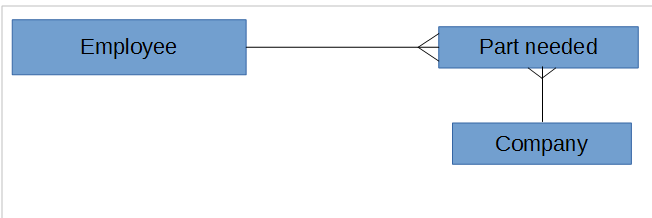
\includegraphics[width =\textwidth]{ERDiagram.jpg}
\end{center}
\subsubsection{Entity Descriptions}
\textbf{Employee}(First Name, Last Name, ID) \\
\textbf{Part Needed}(Part Name, Part Size, Part Price) \\
\textbf{Company Information}(Company Name, Email Address, Telephone Number, Website, Company Owner)  \\
\subsubsection{1NF to 3NF}
\bf{1NF}\\
Non repeating\\
\newline
\underline{UserID}\\
CompanyName\\
OwnerName\\
TelephoneNumber\\
Email\\
Address\\
Website\\
\newline
Repeating\\
\newline
\underline{PartID}\\
\underline{CompanyID}\\
Parts\\
PartPrices\\
PartsProvided\\
Comment\\
Ratings\\
\newline
\bf{2NF}\\
\underline{CompanyID}\\
Comments\\
Ratings\\
\newline
\underline{PartID}\\
Parts\\
\newline
\underline{PartID}\\
\underline{companyID}\\
PartPrices\\
PartsProvided\\
\newline
\bf{3NF}\\
\underline{CompanyParts}\\
PartsProvided\\
PartPrices\\

\subsection{SQL Queries}

\section{Security and Integrity of the System and Data}

\subsection{Security and Integrity of Data}
The system will have no encryption or security as all of the data stored is available to the public anyway either via the internet or advertisements. Therefore there is no need for security as non of the information is private or confidential.

\section{Validation}
Most of the data entered will be strings so not much validation is needed. However for data items such as emails and telephone numbers will need a validation as they are unique. For example, an email entered will have to be checked to see if there is an @ and a . within the string entered.

\section{Testing}

\begin{landscape}
\subsection{Outline Plan}

\begin{center}
    \begin{tabular}{|p{2cm}|p{5cm}|p{5cm}|p{4cm}|}
        \hline
        \textbf{Test Series} & \textbf{Purpose of Test Series} & \textbf{Testing Strategy} & \textbf{Strategy Rationale}\\ \hline
        1 & Test that the user interfaces work and connect with following windows correctly & Top down testing & After the interfaces have been coded, check to see if all of the windows look as planned and any features such as buttons work. \\ \hline
        2 & Test data entered is valid & bottom up testing & Every data item entered will be checked for specific items \\ \hline
        3 & Test that the data is stored in the correct place in the database & black box testing & Once data has been added to the database, check that it has been placed in the right column in the correct table.\\ \hline
        4 & Test that the system meets the full specification & acceptance testing & Once the program has been completed, the client will review it and make sure it has met the full specification.\\ \hline
    \end{tabular}
\end{center}

\subsection{Detailed Plan}

\begin{center}
    \begin{longtable}{|p{1.5cm}|p{2.5cm}|p{2.5cm}|p{2cm}|p{2cm}|p{2cm}|p{2cm}|p{2cm}|}
        \hline
        \textbf{Test Series} & \textbf{Purpose of Test} & \textbf{Test Description} & \textbf{Test Data} & \textbf{Test Data Type (Normal/ Erroneous/ Boundary)} & \textbf{Expected Result} & \textbf{Actual Result} & \textbf{Evidence}\\ \hline
        1.01 & Test Search button works & This should take the data item entered in the search bar and open the results window, closing the main menu window in the process. Search results for the data item entered should be displayed. & Enter an item into the search bar and click the search button & Normal & Results window should show with relevant results &  &  \\ \hline
        1.02 & Test exit button works & This button should exit the program when clicked & Click the exit button & Normal & The program should exit &  &  \\ \hline
        1.03 & Test Add supplier button works & This should take the user to the add information page and close the results window. & Click the add supplier button & Normal & The add information page should display &  &  \\ \hline
       	1.04 & Test the back button works & This should take the user back to the previous window, closing the current window & Click the back button & Normal & The previous window should display and the window the user was on should close. &  &  \\ \hline
       	1.05 & Test the add information line edits work & These should allow the user to input information to be added to the database  & When the add information button has been clicked, the information in the line edits should be added to the database & Add data to the line edits & Normal & Check to see the information from the line edits has been added to the database &  &  \\ \hline
       	1.06 & Test the add information button works & This should add the data from the line edits to the database & Click the button & Normal & The data should be added to the database. &  & \\ \hline
       	1.07 & Test that the edit information button works & This allows the user to edit previously entered information or delete it altogether by taking them to a separate window & Click the edit data button & Normal & The edit data window opens and the previous window closes. & & \\ \hline
       	1.08 Test the edit data line edits function correctly & This should take data from the user to be used to update the information in the database & Add relevant information to the line edits & Normal & The data entered should be added to the database once the update button has been clicked &  &  \\ \hline
       	1.09 Check to see the update button works & Updates the information in the database with the information entered & Click the update button & Normal & The information in the database should be updated with the new information &  &  \\ \hline
       	1.10 Check to see the delete supplier button works & this should delete the whole supplier and all the relevant information about the supplier & Click the delete supplier button & Normal & The supplier and relevant information should be removed from the database &  &  \\ \hline
       	1.11 Test to see if the view comments button works & Show the comments window & Click the view comments button & normal & The comments window should open and the previous window should close & &\\ \hline
       	1.12 Test to see if the add a new comment button works & Shows the add comment window & Click the add a new comment button & normal & The add a new comment window should open and the view comments window should close & &\\ \hline
       	1.13 Test to see if the add comment line edit works & Should allow the user to add their comment to the database & Type in the line edit & Normal & The comment the user typed in should be added to the database once the add comment button has been clicked & & \\ \hline
       	1.14 Check to see if the ratings scroll box works & It should allow the user to scroll through ratings 0 to 10 & Scroll through the scroll box & Normal & the rating the user has scrolled to should be added to the database once the add comment button has been clicked & & \\ \hline
       	1.15 Check to see if the add comment button works & Should add all of the data entered to the database & click the add comment button & The data entered should now be stored in the database & & \\ \hline
       	1.16 Test to see if the edit comments button works & Should open up the edit comments window & Click the edit comments button & normal & The edit comments window should open and the view comments window should close & & \\ \hline
       	1.17 Check to see if the edit comment line edit works & Should allow the user to input the updated comment & Type in the line edit & normal & The information typed in should be added to the database when the update comments button is clicked & & \\ \hline
       	1.18 Test to see if the update comments button works & 
       	
    \end{longtable}
\end{center}
\end{landscape}